% !Mode:: "TeX:UTF-8"
\section{课题来源及研究的背景和意义}
\subsection{课题的来源}

服务被定义为客户、提供者、使能者多方之间协同生产~(co-production)~共创价值的过程。例如,软件化服务(如~Web Service)~ 是软件客户端与服务端通过标准化协议(如~SOAP~协议)的交互,客户端发出请求,服务端执行计算任务并将结果返回给客户端;业务服务是现实中的客户方企业与各服务提供企业之间的交互,这种交互既可以是~Internet~支持的网络交互,也可以是现实中的交互。

这意味着,在业务层面上,服务中的任何一方都无法完全控制全局,服务的执行是一个分布式协作的过程。由于无法全局控制,服务的执行不可避免的要面临各种不确定性,不受某一方控制的服务环节可能无法按照其预设的期望来执行。同样,在软件层面上,由于互联网环境的动态变化和不稳定特性,构建在其基础上的服务系统在执行过程中也面临各种不确定性,某些服务环节可能无法按照预期执行,供需双方期望的价值无法完全实现,还可能触发其他更多的不确定性事件,造成各种直接和潜在的影响。

\subsection{课题研究的背景和意义}
本课题将不确定性定义为“某个已经或即将发生的事件,它使得服务实际执行结果与预先达成的服务级别协议~(Service Level Agreement, SLA)~之间产生了偏差”。服务执行中典型的不确定性包括:
1)~某个服务环节未达到期望的质量~(QoS)~;
2)~某个服务环节执行失败;
3)~客户需求发生变更或完全取消;
4)~可用软件服务或服务资源的数量/价格发生波动;
5)~外部商业环境或政策发生了变化,导致预设的服务流程失效;等等。
从发生时间看,不确定性分为两种类型:已经发生并已造成影响的不确定性、明确知道将要发生但尚未发生的不确定性。

以民航服务为例。某航班遵循预先制定的时间表进行飞行,乘客、航空售票、机场等其他服务参与者规划各自的活动。如果因为机械故障原因导致航班延误(“变”),那么航空公司、售票处、机场、乘客的行为均要随之发生变化,航空公司要根据客户的需求(“需”)指示机场对其进行改签并安排食宿,或要求售票处办理退票、补偿,或者什么也不做(“应”)。这三种对策所造成的后果是不同的,需要根据航班延误的时间长度、涉及乘客的数目等复杂因素动态寻求最优决策。

在服务执行过程中,对发生的不同类型的不确定性事件可能有多种处理对策(重试、补偿、重组、替换等),不同的对策对服务的影响是不同的。如何以最小的代价使服务尽快回到期望轨道,需要做出最优的选择。另外,由于不确定性是可传播的,选择决策时不能仅考虑到对当前环节的处理,还需要考虑到它对未来的长期影响,从而达到整体最优,因此这是一个长期的动态决策过程,其示意图如图~\ref{uc_plan}~所示。

\begin{figure}[htbp]
\centering
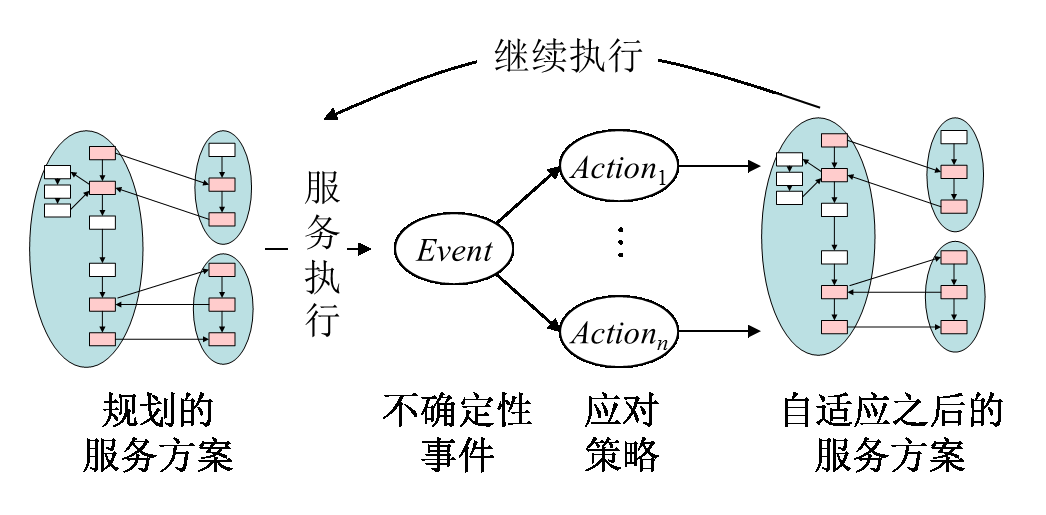
\includegraphics[width = 0.5\textwidth]{uc_plan}
\caption{按需应变的服务不确定性自适应决策}\label{uc_plan}
\vspace{-1em}
\end{figure}

%为了应对不确定性,核心策略就是“按需应变”:根据预期发生的或已经发生的不确定性,对服务做出调整。这里的“变”即各种不确定性事件,“应”即所采取的对策,而“需”则是指在决定采取何种对策时应考虑客户/提供者的特征。按需应变的目标是:以最小的代价,使不确定造成的损失最小化。由于不确定性的动态性,所采取的应对策略也不可能是提前计划好的静态策略,需要根据服务执行时的具体情况选取最优的应对策略。

因此,对服务不确定性进行分析和建模,在服务执行时出现不确定性时以最小的代价将服务恢复至正常状态,并且使得此正常状态后得以成功执行的价值最高,这将避免在服务出现不确定情况时而临时采取对策而造成过高的代价,从而提升顾客满意度。

软件层的服务不确定性较为单一,主要包括服务不可用、延时、执行失败,而在业务层面不仅具有软件层面的服务不确定性事件,还包括用户需求的变化和服务资源变化。由此将导致业务层面的决策方法也同时包括但不限于软件层面不确定性的决策方法,同时需要处理用户需求以及资源变化带来的不确定性。因此,由于软件层面和业务层面的服务不确定性具有很大差别,本课题将分别建立软件层面和业务层面的服务不确定性建模,并采用不同的决策方法。

%本文根据服务执行中发生的具体不确定性,利用不确定性触发关系图(UTG)刻画不确定性事件所导致的服务状态以及所采取的决策动作之间的转换关系,以服务成功执行的概率最大、时间延迟最小、成本最低作为决策优化的目标,建立基于Markov 决策过程(MDP) 的不确定性优化决策模型并加以求解,生成对当前服务方案的最优改进策略。
